% Created by tikzDevice version 0.12.3.1 on 2023-11-03 10:48:16
% !TEX encoding = UTF-8 Unicode
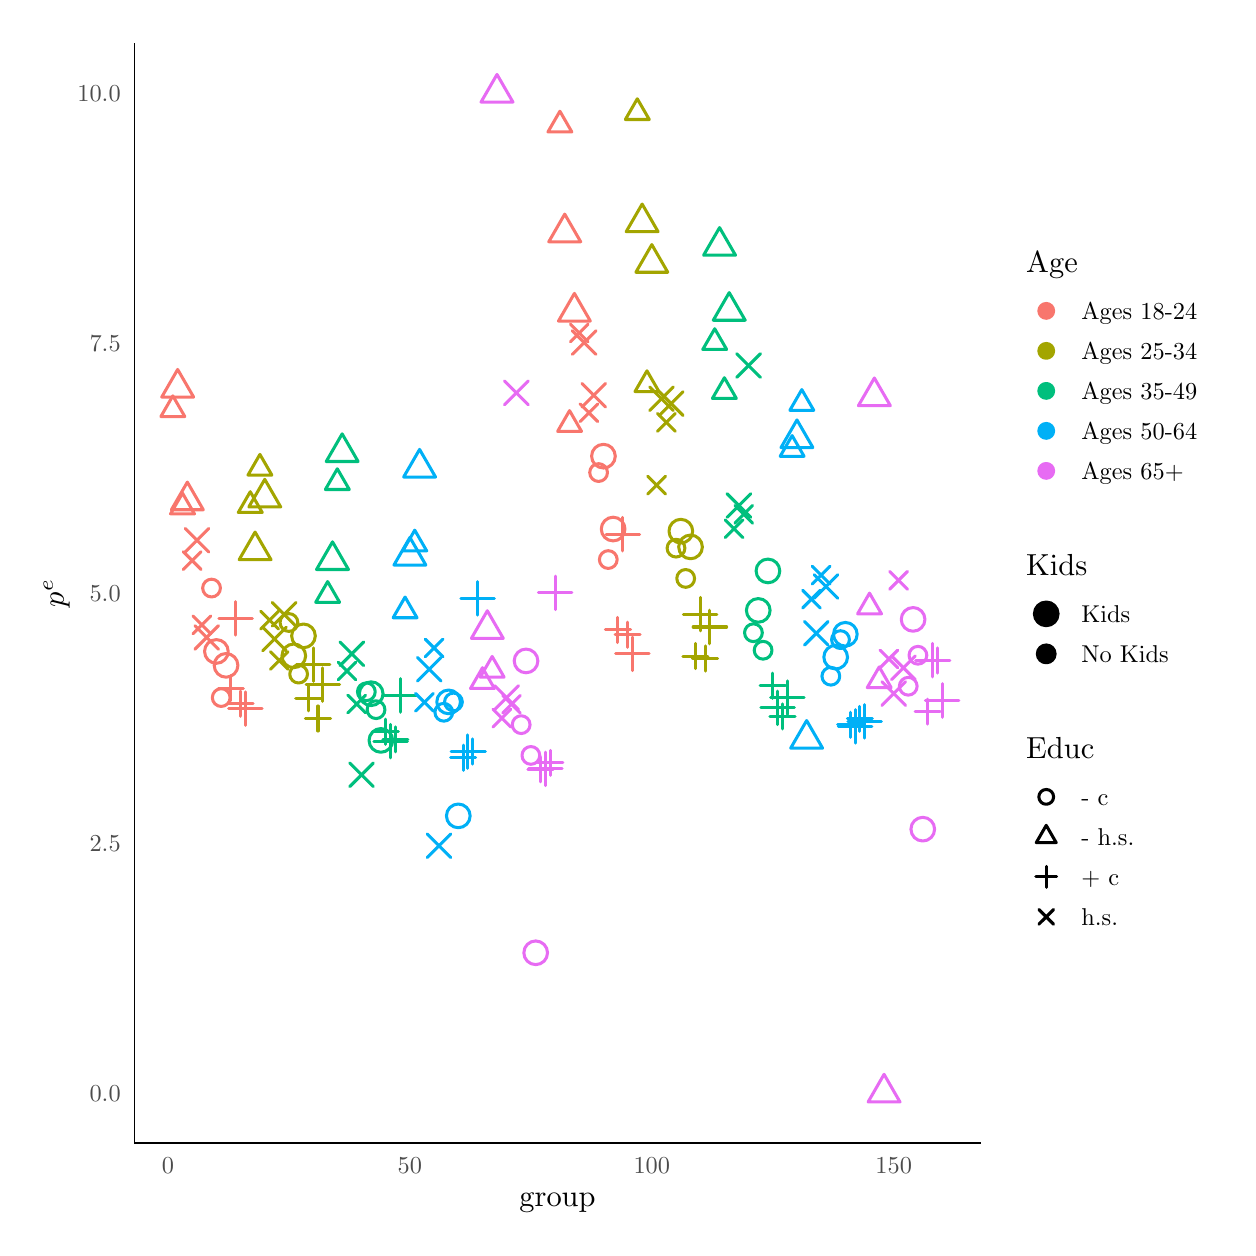
\begin{tikzpicture}[x=1pt,y=1pt]
\definecolor{fillColor}{RGB}{255,255,255}
\path[use as bounding box,fill=fillColor,fill opacity=0.00] (0,0) rectangle (433.62,433.62);
\begin{scope}
\path[clip] ( 38.56, 30.69) rectangle (344.33,428.12);
\definecolor{drawColor}{RGB}{248,118,109}

\path[draw=drawColor,line width= 1.1pt,line join=round,line cap=round] ( 52.45,300.57) --
	( 56.78,293.09) --
	( 48.13,293.09) --
	cycle;

\path[draw=drawColor,line width= 1.1pt,line join=round,line cap=round] ( 54.20,310.11) --
	( 59.97,300.13) --
	( 48.44,300.13) --
	cycle;

\path[draw=drawColor,line width= 1.1pt,line join=round,line cap=round] ( 55.95,265.41) --
	( 60.27,257.92) --
	( 51.63,257.92) --
	cycle;

\path[draw=drawColor,line width= 1.1pt,line join=round,line cap=round] ( 57.70,269.40) --
	( 63.46,259.41) --
	( 51.93,259.41) --
	cycle;

\path[draw=drawColor,line width= 1.1pt,line join=round,line cap=round] ( 56.24,237.85) -- ( 62.66,244.27);

\path[draw=drawColor,line width= 1.1pt,line join=round,line cap=round] ( 56.24,244.27) -- ( 62.66,237.85);

\path[draw=drawColor,line width= 1.1pt,line join=round,line cap=round] ( 56.92,244.13) -- ( 65.48,252.69);

\path[draw=drawColor,line width= 1.1pt,line join=round,line cap=round] ( 56.92,252.69) -- ( 65.48,244.13);

\path[draw=drawColor,line width= 1.1pt,line join=round,line cap=round] ( 59.73,214.58) -- ( 66.15,221.00);

\path[draw=drawColor,line width= 1.1pt,line join=round,line cap=round] ( 59.73,221.00) -- ( 66.15,214.58);

\path[draw=drawColor,line width= 1.1pt,line join=round,line cap=round] ( 60.41,209.00) -- ( 68.97,217.56);

\path[draw=drawColor,line width= 1.1pt,line join=round,line cap=round] ( 60.41,217.56) -- ( 68.97,209.00);

\path[draw=drawColor,line width= 1.1pt,line join=round,line cap=round] ( 66.44,231.12) circle (  3.21);

\path[draw=drawColor,line width= 1.1pt,line join=round,line cap=round] ( 68.19,208.22) circle (  4.28);

\path[draw=drawColor,line width= 1.1pt,line join=round,line cap=round] ( 69.94,191.55) circle (  3.21);

\path[draw=drawColor,line width= 1.1pt,line join=round,line cap=round] ( 71.68,203.19) circle (  4.28);

\path[draw=drawColor,line width= 1.1pt,line join=round,line cap=round] ( 68.89,194.94) -- ( 77.97,194.94);

\path[draw=drawColor,line width= 1.1pt,line join=round,line cap=round] ( 73.43,190.40) -- ( 73.43,199.48);

\path[draw=drawColor,line width= 1.1pt,line join=round,line cap=round] ( 69.13,220.20) -- ( 81.23,220.20);

\path[draw=drawColor,line width= 1.1pt,line join=round,line cap=round] ( 75.18,214.15) -- ( 75.18,226.25);

\path[draw=drawColor,line width= 1.1pt,line join=round,line cap=round] ( 72.39,189.34) -- ( 81.47,189.34);

\path[draw=drawColor,line width= 1.1pt,line join=round,line cap=round] ( 76.93,184.80) -- ( 76.93,193.88);

\path[draw=drawColor,line width= 1.1pt,line join=round,line cap=round] ( 72.63,187.56) -- ( 84.73,187.56);

\path[draw=drawColor,line width= 1.1pt,line join=round,line cap=round] ( 78.68,181.50) -- ( 78.68,193.61);
\definecolor{drawColor}{RGB}{163,165,0}

\path[draw=drawColor,line width= 1.1pt,line join=round,line cap=round] ( 80.43,265.93) --
	( 84.75,258.44) --
	( 76.10,258.44) --
	cycle;

\path[draw=drawColor,line width= 1.1pt,line join=round,line cap=round] ( 82.17,251.35) --
	( 87.94,241.37) --
	( 76.41,241.37) --
	cycle;

\path[draw=drawColor,line width= 1.1pt,line join=round,line cap=round] ( 83.92,279.42) --
	( 88.24,271.94) --
	( 79.60,271.94) --
	cycle;

\path[draw=drawColor,line width= 1.1pt,line join=round,line cap=round] ( 85.67,270.41) --
	( 91.43,260.43) --
	( 79.91,260.43) --
	cycle;

\path[draw=drawColor,line width= 1.1pt,line join=round,line cap=round] ( 84.21,216.33) -- ( 90.63,222.75);

\path[draw=drawColor,line width= 1.1pt,line join=round,line cap=round] ( 84.21,222.75) -- ( 90.63,216.33);

\path[draw=drawColor,line width= 1.1pt,line join=round,line cap=round] ( 84.89,208.45) -- ( 93.45,217.01);

\path[draw=drawColor,line width= 1.1pt,line join=round,line cap=round] ( 84.89,217.01) -- ( 93.45,208.45);

\path[draw=drawColor,line width= 1.1pt,line join=round,line cap=round] ( 87.71,201.74) -- ( 94.12,208.15);

\path[draw=drawColor,line width= 1.1pt,line join=round,line cap=round] ( 87.71,208.15) -- ( 94.12,201.74);

\path[draw=drawColor,line width= 1.1pt,line join=round,line cap=round] ( 88.38,217.36) -- ( 96.94,225.92);

\path[draw=drawColor,line width= 1.1pt,line join=round,line cap=round] ( 88.38,225.92) -- ( 96.94,217.36);

\path[draw=drawColor,line width= 1.1pt,line join=round,line cap=round] ( 94.41,218.67) circle (  3.21);

\path[draw=drawColor,line width= 1.1pt,line join=round,line cap=round] ( 96.16,206.63) circle (  4.28);

\path[draw=drawColor,line width= 1.1pt,line join=round,line cap=round] ( 97.91,200.03) circle (  3.21);

\path[draw=drawColor,line width= 1.1pt,line join=round,line cap=round] ( 99.66,213.84) circle (  4.28);

\path[draw=drawColor,line width= 1.1pt,line join=round,line cap=round] ( 96.87,191.24) -- (105.94,191.24);

\path[draw=drawColor,line width= 1.1pt,line join=round,line cap=round] (101.41,186.71) -- (101.41,195.78);

\path[draw=drawColor,line width= 1.1pt,line join=round,line cap=round] ( 97.10,203.45) -- (109.21,203.45);

\path[draw=drawColor,line width= 1.1pt,line join=round,line cap=round] (103.15,197.40) -- (103.15,209.50);

\path[draw=drawColor,line width= 1.1pt,line join=round,line cap=round] (100.36,183.98) -- (109.44,183.98);

\path[draw=drawColor,line width= 1.1pt,line join=round,line cap=round] (104.90,179.45) -- (104.90,188.52);

\path[draw=drawColor,line width= 1.1pt,line join=round,line cap=round] (100.60,196.22) -- (112.70,196.22);

\path[draw=drawColor,line width= 1.1pt,line join=round,line cap=round] (106.65,190.17) -- (106.65,202.27);
\definecolor{drawColor}{RGB}{0,191,125}

\path[draw=drawColor,line width= 1.1pt,line join=round,line cap=round] (108.40,233.46) --
	(112.72,225.97) --
	(104.08,225.97) --
	cycle;

\path[draw=drawColor,line width= 1.1pt,line join=round,line cap=round] (110.15,247.82) --
	(115.91,237.83) --
	(104.38,237.83) --
	cycle;

\path[draw=drawColor,line width= 1.1pt,line join=round,line cap=round] (111.89,274.22) --
	(116.22,266.73) --
	(107.57,266.73) --
	cycle;

\path[draw=drawColor,line width= 1.1pt,line join=round,line cap=round] (113.64,286.84) --
	(119.41,276.85) --
	(107.88,276.85) --
	cycle;

\path[draw=drawColor,line width= 1.1pt,line join=round,line cap=round] (112.18,197.95) -- (118.60,204.37);

\path[draw=drawColor,line width= 1.1pt,line join=round,line cap=round] (112.18,204.37) -- (118.60,197.95);

\path[draw=drawColor,line width= 1.1pt,line join=round,line cap=round] (112.86,203.09) -- (121.42,211.65);

\path[draw=drawColor,line width= 1.1pt,line join=round,line cap=round] (112.86,211.65) -- (121.42,203.09);

\path[draw=drawColor,line width= 1.1pt,line join=round,line cap=round] (115.68,186.02) -- (122.10,192.44);

\path[draw=drawColor,line width= 1.1pt,line join=round,line cap=round] (115.68,192.44) -- (122.10,186.02);

\path[draw=drawColor,line width= 1.1pt,line join=round,line cap=round] (116.36,159.36) -- (124.92,167.92);

\path[draw=drawColor,line width= 1.1pt,line join=round,line cap=round] (116.36,167.92) -- (124.92,159.36);

\path[draw=drawColor,line width= 1.1pt,line join=round,line cap=round] (122.38,193.64) circle (  3.21);

\path[draw=drawColor,line width= 1.1pt,line join=round,line cap=round] (124.13,192.95) circle (  4.28);

\path[draw=drawColor,line width= 1.1pt,line join=round,line cap=round] (125.88,187.18) circle (  3.21);

\path[draw=drawColor,line width= 1.1pt,line join=round,line cap=round] (127.63,176.07) circle (  4.28);

\path[draw=drawColor,line width= 1.1pt,line join=round,line cap=round] (124.84,179.18) -- (133.92,179.18);

\path[draw=drawColor,line width= 1.1pt,line join=round,line cap=round] (129.38,174.64) -- (129.38,183.72);

\path[draw=drawColor,line width= 1.1pt,line join=round,line cap=round] (125.07,175.84) -- (137.18,175.84);

\path[draw=drawColor,line width= 1.1pt,line join=round,line cap=round] (131.13,169.79) -- (131.13,181.89);

\path[draw=drawColor,line width= 1.1pt,line join=round,line cap=round] (128.34,176.45) -- (137.41,176.45);

\path[draw=drawColor,line width= 1.1pt,line join=round,line cap=round] (132.87,171.91) -- (132.87,180.99);

\path[draw=drawColor,line width= 1.1pt,line join=round,line cap=round] (128.57,192.30) -- (140.68,192.30);

\path[draw=drawColor,line width= 1.1pt,line join=round,line cap=round] (134.62,186.25) -- (134.62,198.36);
\definecolor{drawColor}{RGB}{0,176,246}

\path[draw=drawColor,line width= 1.1pt,line join=round,line cap=round] (136.37,227.87) --
	(140.69,220.39) --
	(132.05,220.39) --
	cycle;

\path[draw=drawColor,line width= 1.1pt,line join=round,line cap=round] (138.12,249.41) --
	(143.88,239.43) --
	(132.35,239.43) --
	cycle;

\path[draw=drawColor,line width= 1.1pt,line join=round,line cap=round] (139.87,252.04) --
	(144.19,244.55) --
	(135.55,244.55) --
	cycle;

\path[draw=drawColor,line width= 1.1pt,line join=round,line cap=round] (141.62,281.22) --
	(147.38,271.24) --
	(135.85,271.24) --
	cycle;

\path[draw=drawColor,line width= 1.1pt,line join=round,line cap=round] (140.15,186.65) -- (146.57,193.06);

\path[draw=drawColor,line width= 1.1pt,line join=round,line cap=round] (140.15,193.06) -- (146.57,186.65);

\path[draw=drawColor,line width= 1.1pt,line join=round,line cap=round] (140.83,197.53) -- (149.39,206.09);

\path[draw=drawColor,line width= 1.1pt,line join=round,line cap=round] (140.83,206.09) -- (149.39,197.53);

\path[draw=drawColor,line width= 1.1pt,line join=round,line cap=round] (143.65,206.26) -- (150.07,212.68);

\path[draw=drawColor,line width= 1.1pt,line join=round,line cap=round] (143.65,212.68) -- (150.07,206.26);

\path[draw=drawColor,line width= 1.1pt,line join=round,line cap=round] (144.33,133.73) -- (152.89,142.29);

\path[draw=drawColor,line width= 1.1pt,line join=round,line cap=round] (144.33,142.29) -- (152.89,133.73);

\path[draw=drawColor,line width= 1.1pt,line join=round,line cap=round] (150.36,186.24) circle (  3.21);

\path[draw=drawColor,line width= 1.1pt,line join=round,line cap=round] (152.11,189.99) circle (  4.28);

\path[draw=drawColor,line width= 1.1pt,line join=round,line cap=round] (153.85,189.97) circle (  3.21);

\path[draw=drawColor,line width= 1.1pt,line join=round,line cap=round] (155.60,148.80) circle (  4.28);

\path[draw=drawColor,line width= 1.1pt,line join=round,line cap=round] (152.81,169.81) -- (161.89,169.81);

\path[draw=drawColor,line width= 1.1pt,line join=round,line cap=round] (157.35,165.27) -- (157.35,174.35);

\path[draw=drawColor,line width= 1.1pt,line join=round,line cap=round] (153.05,172.03) -- (165.15,172.03);

\path[draw=drawColor,line width= 1.1pt,line join=round,line cap=round] (159.10,165.98) -- (159.10,178.08);

\path[draw=drawColor,line width= 1.1pt,line join=round,line cap=round] (156.31,172.06) -- (165.38,172.06);

\path[draw=drawColor,line width= 1.1pt,line join=round,line cap=round] (160.85,167.52) -- (160.85,176.59);

\path[draw=drawColor,line width= 1.1pt,line join=round,line cap=round] (156.54,227.40) -- (168.65,227.40);

\path[draw=drawColor,line width= 1.1pt,line join=round,line cap=round] (162.59,221.34) -- (162.59,233.45);
\definecolor{drawColor}{RGB}{231,107,243}

\path[draw=drawColor,line width= 1.1pt,line join=round,line cap=round] (164.34,202.33) --
	(168.66,194.84) --
	(160.02,194.84) --
	cycle;

\path[draw=drawColor,line width= 1.1pt,line join=round,line cap=round] (166.09,222.92) --
	(171.86,212.94) --
	(160.33,212.94) --
	cycle;

\path[draw=drawColor,line width= 1.1pt,line join=round,line cap=round] (167.84,206.41) --
	(172.16,198.93) --
	(163.52,198.93) --
	cycle;

\path[draw=drawColor,line width= 1.1pt,line join=round,line cap=round] (169.59,416.71) --
	(175.35,406.73) --
	(163.82,406.73) --
	cycle;

\path[draw=drawColor,line width= 1.1pt,line join=round,line cap=round] (168.13,180.90) -- (174.54,187.31);

\path[draw=drawColor,line width= 1.1pt,line join=round,line cap=round] (168.13,187.31) -- (174.54,180.90);

\path[draw=drawColor,line width= 1.1pt,line join=round,line cap=round] (168.80,187.26) -- (177.36,195.82);

\path[draw=drawColor,line width= 1.1pt,line join=round,line cap=round] (168.80,195.82) -- (177.36,187.26);

\path[draw=drawColor,line width= 1.1pt,line join=round,line cap=round] (171.62,185.94) -- (178.04,192.36);

\path[draw=drawColor,line width= 1.1pt,line join=round,line cap=round] (171.62,192.36) -- (178.04,185.94);

\path[draw=drawColor,line width= 1.1pt,line join=round,line cap=round] (172.30,297.38) -- (180.86,305.94);

\path[draw=drawColor,line width= 1.1pt,line join=round,line cap=round] (172.30,305.94) -- (180.86,297.38);

\path[draw=drawColor,line width= 1.1pt,line join=round,line cap=round] (178.33,181.77) circle (  3.21);

\path[draw=drawColor,line width= 1.1pt,line join=round,line cap=round] (180.08,204.79) circle (  4.28);

\path[draw=drawColor,line width= 1.1pt,line join=round,line cap=round] (181.83,170.64) circle (  3.21);

\path[draw=drawColor,line width= 1.1pt,line join=round,line cap=round] (183.57, 99.33) circle (  4.28);

\path[draw=drawColor,line width= 1.1pt,line join=round,line cap=round] (180.78,165.59) -- (189.86,165.59);

\path[draw=drawColor,line width= 1.1pt,line join=round,line cap=round] (185.32,161.05) -- (185.32,170.13);

\path[draw=drawColor,line width= 1.1pt,line join=round,line cap=round] (181.02,165.78) -- (193.12,165.78);

\path[draw=drawColor,line width= 1.1pt,line join=round,line cap=round] (187.07,159.73) -- (187.07,171.83);

\path[draw=drawColor,line width= 1.1pt,line join=round,line cap=round] (184.28,167.94) -- (193.36,167.94);

\path[draw=drawColor,line width= 1.1pt,line join=round,line cap=round] (188.82,163.40) -- (188.82,172.48);

\path[draw=drawColor,line width= 1.1pt,line join=round,line cap=round] (184.51,229.40) -- (196.62,229.40);

\path[draw=drawColor,line width= 1.1pt,line join=round,line cap=round] (190.57,223.35) -- (190.57,235.46);
\definecolor{drawColor}{RGB}{248,118,109}

\path[draw=drawColor,line width= 1.1pt,line join=round,line cap=round] (192.32,403.42) --
	(196.64,395.93) --
	(187.99,395.93) --
	cycle;

\path[draw=drawColor,line width= 1.1pt,line join=round,line cap=round] (194.06,366.24) --
	(199.83,356.25) --
	(188.30,356.25) --
	cycle;

\path[draw=drawColor,line width= 1.1pt,line join=round,line cap=round] (195.81,295.23) --
	(200.13,287.74) --
	(191.49,287.74) --
	cycle;

\path[draw=drawColor,line width= 1.1pt,line join=round,line cap=round] (197.56,337.59) --
	(203.32,327.60) --
	(191.80,327.60) --
	cycle;

\path[draw=drawColor,line width= 1.1pt,line join=round,line cap=round] (196.10,320.10) -- (202.52,326.52);

\path[draw=drawColor,line width= 1.1pt,line join=round,line cap=round] (196.10,326.52) -- (202.52,320.10);

\path[draw=drawColor,line width= 1.1pt,line join=round,line cap=round] (196.78,315.55) -- (205.34,324.11);

\path[draw=drawColor,line width= 1.1pt,line join=round,line cap=round] (196.78,324.11) -- (205.34,315.55);

\path[draw=drawColor,line width= 1.1pt,line join=round,line cap=round] (199.60,291.25) -- (206.01,297.67);

\path[draw=drawColor,line width= 1.1pt,line join=round,line cap=round] (199.60,297.67) -- (206.01,291.25);

\path[draw=drawColor,line width= 1.1pt,line join=round,line cap=round] (200.27,296.54) -- (208.83,305.10);

\path[draw=drawColor,line width= 1.1pt,line join=round,line cap=round] (200.27,305.10) -- (208.83,296.54);

\path[draw=drawColor,line width= 1.1pt,line join=round,line cap=round] (206.30,272.86) circle (  3.21);

\path[draw=drawColor,line width= 1.1pt,line join=round,line cap=round] (208.05,278.78) circle (  4.28);

\path[draw=drawColor,line width= 1.1pt,line join=round,line cap=round] (209.80,241.42) circle (  3.21);

\path[draw=drawColor,line width= 1.1pt,line join=round,line cap=round] (211.55,252.44) circle (  4.28);

\path[draw=drawColor,line width= 1.1pt,line join=round,line cap=round] (208.76,215.98) -- (217.83,215.98);

\path[draw=drawColor,line width= 1.1pt,line join=round,line cap=round] (213.29,211.45) -- (213.29,220.52);

\path[draw=drawColor,line width= 1.1pt,line join=round,line cap=round] (208.99,250.58) -- (221.10,250.58);

\path[draw=drawColor,line width= 1.1pt,line join=round,line cap=round] (215.04,244.52) -- (215.04,256.63);

\path[draw=drawColor,line width= 1.1pt,line join=round,line cap=round] (212.25,214.26) -- (221.33,214.26);

\path[draw=drawColor,line width= 1.1pt,line join=round,line cap=round] (216.79,209.73) -- (216.79,218.80);

\path[draw=drawColor,line width= 1.1pt,line join=round,line cap=round] (212.49,207.36) -- (224.59,207.36);

\path[draw=drawColor,line width= 1.1pt,line join=round,line cap=round] (218.54,201.30) -- (218.54,213.41);
\definecolor{drawColor}{RGB}{163,165,0}

\path[draw=drawColor,line width= 1.1pt,line join=round,line cap=round] (220.29,407.92) --
	(224.61,400.43) --
	(215.97,400.43) --
	cycle;

\path[draw=drawColor,line width= 1.1pt,line join=round,line cap=round] (222.04,369.88) --
	(227.80,359.90) --
	(216.27,359.90) --
	cycle;

\path[draw=drawColor,line width= 1.1pt,line join=round,line cap=round] (223.78,309.62) --
	(228.11,302.13) --
	(219.46,302.13) --
	cycle;

\path[draw=drawColor,line width= 1.1pt,line join=round,line cap=round] (225.53,355.22) --
	(231.30,345.24) --
	(219.77,345.24) --
	cycle;

\path[draw=drawColor,line width= 1.1pt,line join=round,line cap=round] (224.07,265.10) -- (230.49,271.52);

\path[draw=drawColor,line width= 1.1pt,line join=round,line cap=round] (224.07,271.52) -- (230.49,265.10);

\path[draw=drawColor,line width= 1.1pt,line join=round,line cap=round] (224.75,295.22) -- (233.31,303.78);

\path[draw=drawColor,line width= 1.1pt,line join=round,line cap=round] (224.75,303.78) -- (233.31,295.22);

\path[draw=drawColor,line width= 1.1pt,line join=round,line cap=round] (227.57,287.76) -- (233.99,294.18);

\path[draw=drawColor,line width= 1.1pt,line join=round,line cap=round] (227.57,294.18) -- (233.99,287.76);

\path[draw=drawColor,line width= 1.1pt,line join=round,line cap=round] (228.25,293.50) -- (236.81,302.06);

\path[draw=drawColor,line width= 1.1pt,line join=round,line cap=round] (228.25,302.06) -- (236.81,293.50);

\path[draw=drawColor,line width= 1.1pt,line join=round,line cap=round] (234.27,245.54) circle (  3.21);

\path[draw=drawColor,line width= 1.1pt,line join=round,line cap=round] (236.02,251.68) circle (  4.28);

\path[draw=drawColor,line width= 1.1pt,line join=round,line cap=round] (237.77,234.60) circle (  3.21);

\path[draw=drawColor,line width= 1.1pt,line join=round,line cap=round] (239.52,245.99) circle (  4.28);

\path[draw=drawColor,line width= 1.1pt,line join=round,line cap=round] (236.73,206.56) -- (245.80,206.56);

\path[draw=drawColor,line width= 1.1pt,line join=round,line cap=round] (241.27,202.02) -- (241.27,211.10);

\path[draw=drawColor,line width= 1.1pt,line join=round,line cap=round] (236.96,221.72) -- (249.07,221.72);

\path[draw=drawColor,line width= 1.1pt,line join=round,line cap=round] (243.01,215.66) -- (243.01,227.77);

\path[draw=drawColor,line width= 1.1pt,line join=round,line cap=round] (240.23,205.65) -- (249.30,205.65);

\path[draw=drawColor,line width= 1.1pt,line join=round,line cap=round] (244.76,201.11) -- (244.76,210.19);

\path[draw=drawColor,line width= 1.1pt,line join=round,line cap=round] (240.46,217.05) -- (252.56,217.05);

\path[draw=drawColor,line width= 1.1pt,line join=round,line cap=round] (246.51,211.00) -- (246.51,223.10);
\definecolor{drawColor}{RGB}{0,191,125}

\path[draw=drawColor,line width= 1.1pt,line join=round,line cap=round] (248.26,324.82) --
	(252.58,317.34) --
	(243.94,317.34) --
	cycle;

\path[draw=drawColor,line width= 1.1pt,line join=round,line cap=round] (250.01,361.37) --
	(255.77,351.39) --
	(244.24,351.39) --
	cycle;

\path[draw=drawColor,line width= 1.1pt,line join=round,line cap=round] (251.76,307.12) --
	(256.08,299.64) --
	(247.43,299.64) --
	cycle;

\path[draw=drawColor,line width= 1.1pt,line join=round,line cap=round] (253.50,337.88) --
	(259.27,327.90) --
	(247.74,327.90) --
	cycle;

\path[draw=drawColor,line width= 1.1pt,line join=round,line cap=round] (252.04,249.33) -- (258.46,255.75);

\path[draw=drawColor,line width= 1.1pt,line join=round,line cap=round] (252.04,255.75) -- (258.46,249.33);

\path[draw=drawColor,line width= 1.1pt,line join=round,line cap=round] (252.72,256.67) -- (261.28,265.23);

\path[draw=drawColor,line width= 1.1pt,line join=round,line cap=round] (252.72,265.23) -- (261.28,256.67);

\path[draw=drawColor,line width= 1.1pt,line join=round,line cap=round] (255.54,254.56) -- (261.96,260.98);

\path[draw=drawColor,line width= 1.1pt,line join=round,line cap=round] (255.54,260.98) -- (261.96,254.56);

\path[draw=drawColor,line width= 1.1pt,line join=round,line cap=round] (256.22,307.25) -- (264.78,315.81);

\path[draw=drawColor,line width= 1.1pt,line join=round,line cap=round] (256.22,315.81) -- (264.78,307.25);

\path[draw=drawColor,line width= 1.1pt,line join=round,line cap=round] (262.25,214.98) circle (  3.21);

\path[draw=drawColor,line width= 1.1pt,line join=round,line cap=round] (263.99,223.05) circle (  4.28);

\path[draw=drawColor,line width= 1.1pt,line join=round,line cap=round] (265.74,208.65) circle (  3.21);

\path[draw=drawColor,line width= 1.1pt,line join=round,line cap=round] (267.49,237.31) circle (  4.28);

\path[draw=drawColor,line width= 1.1pt,line join=round,line cap=round] (264.70,195.84) -- (273.78,195.84);

\path[draw=drawColor,line width= 1.1pt,line join=round,line cap=round] (269.24,191.30) -- (269.24,200.37);

\path[draw=drawColor,line width= 1.1pt,line join=round,line cap=round] (264.93,187.80) -- (277.04,187.80);

\path[draw=drawColor,line width= 1.1pt,line join=round,line cap=round] (270.99,181.75) -- (270.99,193.85);

\path[draw=drawColor,line width= 1.1pt,line join=round,line cap=round] (268.20,184.73) -- (277.27,184.73);

\path[draw=drawColor,line width= 1.1pt,line join=round,line cap=round] (272.74,180.20) -- (272.74,189.27);

\path[draw=drawColor,line width= 1.1pt,line join=round,line cap=round] (268.43,191.51) -- (280.54,191.51);

\path[draw=drawColor,line width= 1.1pt,line join=round,line cap=round] (274.48,185.45) -- (274.48,197.56);
\definecolor{drawColor}{RGB}{0,176,246}

\path[draw=drawColor,line width= 1.1pt,line join=round,line cap=round] (276.23,286.22) --
	(280.55,278.73) --
	(271.91,278.73) --
	cycle;

\path[draw=drawColor,line width= 1.1pt,line join=round,line cap=round] (277.98,291.87) --
	(283.74,281.89) --
	(272.22,281.89) --
	cycle;

\path[draw=drawColor,line width= 1.1pt,line join=round,line cap=round] (279.73,302.83) --
	(284.05,295.35) --
	(275.41,295.35) --
	cycle;

\path[draw=drawColor,line width= 1.1pt,line join=round,line cap=round] (281.48,183.25) --
	(287.24,173.27) --
	(275.71,173.27) --
	cycle;

\path[draw=drawColor,line width= 1.1pt,line join=round,line cap=round] (280.02,223.91) -- (286.43,230.33);

\path[draw=drawColor,line width= 1.1pt,line join=round,line cap=round] (280.02,230.33) -- (286.43,223.91);

\path[draw=drawColor,line width= 1.1pt,line join=round,line cap=round] (280.69,210.49) -- (289.25,219.04);

\path[draw=drawColor,line width= 1.1pt,line join=round,line cap=round] (280.69,219.04) -- (289.25,210.49);

\path[draw=drawColor,line width= 1.1pt,line join=round,line cap=round] (283.51,232.58) -- (289.93,239.00);

\path[draw=drawColor,line width= 1.1pt,line join=round,line cap=round] (283.51,239.00) -- (289.93,232.58);

\path[draw=drawColor,line width= 1.1pt,line join=round,line cap=round] (284.19,227.38) -- (292.75,235.94);

\path[draw=drawColor,line width= 1.1pt,line join=round,line cap=round] (284.19,235.94) -- (292.75,227.38);

\path[draw=drawColor,line width= 1.1pt,line join=round,line cap=round] (290.22,199.27) circle (  3.21);

\path[draw=drawColor,line width= 1.1pt,line join=round,line cap=round] (291.97,206.16) circle (  4.28);

\path[draw=drawColor,line width= 1.1pt,line join=round,line cap=round] (293.71,212.49) circle (  3.21);

\path[draw=drawColor,line width= 1.1pt,line join=round,line cap=round] (295.46,214.42) circle (  4.28);

\path[draw=drawColor,line width= 1.1pt,line join=round,line cap=round] (292.67,181.70) -- (301.75,181.70);

\path[draw=drawColor,line width= 1.1pt,line join=round,line cap=round] (297.21,177.16) -- (297.21,186.24);

\path[draw=drawColor,line width= 1.1pt,line join=round,line cap=round] (292.91,181.16) -- (305.01,181.16);

\path[draw=drawColor,line width= 1.1pt,line join=round,line cap=round] (298.96,175.11) -- (298.96,187.22);

\path[draw=drawColor,line width= 1.1pt,line join=round,line cap=round] (296.17,183.86) -- (305.25,183.86);

\path[draw=drawColor,line width= 1.1pt,line join=round,line cap=round] (300.71,179.33) -- (300.71,188.40);

\path[draw=drawColor,line width= 1.1pt,line join=round,line cap=round] (296.40,182.95) -- (308.51,182.95);

\path[draw=drawColor,line width= 1.1pt,line join=round,line cap=round] (302.46,176.90) -- (302.46,189.00);
\definecolor{drawColor}{RGB}{231,107,243}

\path[draw=drawColor,line width= 1.1pt,line join=round,line cap=round] (304.20,229.29) --
	(308.53,221.80) --
	(299.88,221.80) --
	cycle;

\path[draw=drawColor,line width= 1.1pt,line join=round,line cap=round] (305.95,307.02) --
	(311.72,297.03) --
	(300.19,297.03) --
	cycle;

\path[draw=drawColor,line width= 1.1pt,line join=round,line cap=round] (307.70,202.63) --
	(312.02,195.15) --
	(303.38,195.15) --
	cycle;

\path[draw=drawColor,line width= 1.1pt,line join=round,line cap=round] (309.45, 55.41) --
	(315.21, 45.42) --
	(303.69, 45.42) --
	cycle;

\path[draw=drawColor,line width= 1.1pt,line join=round,line cap=round] (307.99,202.29) -- (314.41,208.70);

\path[draw=drawColor,line width= 1.1pt,line join=round,line cap=round] (307.99,208.70) -- (314.41,202.29);

\path[draw=drawColor,line width= 1.1pt,line join=round,line cap=round] (308.67,188.71) -- (317.23,197.27);

\path[draw=drawColor,line width= 1.1pt,line join=round,line cap=round] (308.67,197.27) -- (317.23,188.71);

\path[draw=drawColor,line width= 1.1pt,line join=round,line cap=round] (311.49,230.71) -- (317.90,237.13);

\path[draw=drawColor,line width= 1.1pt,line join=round,line cap=round] (311.49,237.13) -- (317.90,230.71);

\path[draw=drawColor,line width= 1.1pt,line join=round,line cap=round] (312.16,198.03) -- (320.72,206.59);

\path[draw=drawColor,line width= 1.1pt,line join=round,line cap=round] (312.16,206.59) -- (320.72,198.03);

\path[draw=drawColor,line width= 1.1pt,line join=round,line cap=round] (318.19,195.64) circle (  3.21);

\path[draw=drawColor,line width= 1.1pt,line join=round,line cap=round] (319.94,219.80) circle (  4.28);

\path[draw=drawColor,line width= 1.1pt,line join=round,line cap=round] (321.69,206.84) circle (  3.21);

\path[draw=drawColor,line width= 1.1pt,line join=round,line cap=round] (323.44,144.00) circle (  4.28);

\path[draw=drawColor,line width= 1.1pt,line join=round,line cap=round] (320.65,186.47) -- (329.72,186.47);

\path[draw=drawColor,line width= 1.1pt,line join=round,line cap=round] (325.18,181.94) -- (325.18,191.01);

\path[draw=drawColor,line width= 1.1pt,line join=round,line cap=round] (320.88,205.04) -- (332.98,205.04);

\path[draw=drawColor,line width= 1.1pt,line join=round,line cap=round] (326.93,198.99) -- (326.93,211.09);

\path[draw=drawColor,line width= 1.1pt,line join=round,line cap=round] (324.14,204.94) -- (333.22,204.94);

\path[draw=drawColor,line width= 1.1pt,line join=round,line cap=round] (328.68,200.40) -- (328.68,209.48);

\path[draw=drawColor,line width= 1.1pt,line join=round,line cap=round] (324.38,190.49) -- (336.48,190.49);

\path[draw=drawColor,line width= 1.1pt,line join=round,line cap=round] (330.43,184.44) -- (330.43,196.55);
\end{scope}
\begin{scope}
\path[clip] (  0.00,  0.00) rectangle (433.62,433.62);
\definecolor{drawColor}{RGB}{0,0,0}

\path[draw=drawColor,line width= 0.6pt,line join=round] ( 38.56, 30.69) --
	( 38.56,428.12);
\end{scope}
\begin{scope}
\path[clip] (  0.00,  0.00) rectangle (433.62,433.62);
\definecolor{drawColor}{gray}{0.30}

\node[text=drawColor,anchor=base east,inner sep=0pt, outer sep=0pt, scale=  0.88] at ( 33.61, 45.72) {0.0};

\node[text=drawColor,anchor=base east,inner sep=0pt, outer sep=0pt, scale=  0.88] at ( 33.61,136.05) {2.5};

\node[text=drawColor,anchor=base east,inner sep=0pt, outer sep=0pt, scale=  0.88] at ( 33.61,226.37) {5.0};

\node[text=drawColor,anchor=base east,inner sep=0pt, outer sep=0pt, scale=  0.88] at ( 33.61,316.70) {7.5};

\node[text=drawColor,anchor=base east,inner sep=0pt, outer sep=0pt, scale=  0.88] at ( 33.61,407.02) {10.0};
\end{scope}
\begin{scope}
\path[clip] (  0.00,  0.00) rectangle (433.62,433.62);
\definecolor{drawColor}{RGB}{0,0,0}

\path[draw=drawColor,line width= 0.6pt,line join=round] ( 38.56, 30.69) --
	(344.33, 30.69);
\end{scope}
\begin{scope}
\path[clip] (  0.00,  0.00) rectangle (433.62,433.62);
\definecolor{drawColor}{gray}{0.30}

\node[text=drawColor,anchor=base,inner sep=0pt, outer sep=0pt, scale=  0.88] at ( 50.71, 19.68) {0};

\node[text=drawColor,anchor=base,inner sep=0pt, outer sep=0pt, scale=  0.88] at (138.12, 19.68) {50};

\node[text=drawColor,anchor=base,inner sep=0pt, outer sep=0pt, scale=  0.88] at (225.53, 19.68) {100};

\node[text=drawColor,anchor=base,inner sep=0pt, outer sep=0pt, scale=  0.88] at (312.95, 19.68) {150};
\end{scope}
\begin{scope}
\path[clip] (  0.00,  0.00) rectangle (433.62,433.62);
\definecolor{drawColor}{RGB}{0,0,0}

\node[text=drawColor,anchor=base,inner sep=0pt, outer sep=0pt, scale=  1.10] at (191.44,  7.64) {group};
\end{scope}
\begin{scope}
\path[clip] (  0.00,  0.00) rectangle (433.62,433.62);
\definecolor{drawColor}{RGB}{0,0,0}

\node[text=drawColor,rotate= 90.00,anchor=base,inner sep=0pt, outer sep=0pt, scale=  1.10] at ( 13.08,229.40) {$p^e$};
\end{scope}
\begin{scope}
\path[clip] (  0.00,  0.00) rectangle (433.62,433.62);
\definecolor{drawColor}{RGB}{0,0,0}

\node[text=drawColor,anchor=base west,inner sep=0pt, outer sep=0pt, scale=  1.10] at (360.83,345.08) {Age};
\end{scope}
\begin{scope}
\path[clip] (  0.00,  0.00) rectangle (433.62,433.62);
\definecolor{drawColor}{RGB}{248,118,109}
\definecolor{fillColor}{RGB}{248,118,109}

\path[draw=drawColor,line width= 1.1pt,line join=round,line cap=round,fill=fillColor] (368.05,331.28) circle (  2.67);
\end{scope}
\begin{scope}
\path[clip] (  0.00,  0.00) rectangle (433.62,433.62);
\definecolor{drawColor}{RGB}{163,165,0}
\definecolor{fillColor}{RGB}{163,165,0}

\path[draw=drawColor,line width= 1.1pt,line join=round,line cap=round,fill=fillColor] (368.05,316.83) circle (  2.67);
\end{scope}
\begin{scope}
\path[clip] (  0.00,  0.00) rectangle (433.62,433.62);
\definecolor{drawColor}{RGB}{0,191,125}
\definecolor{fillColor}{RGB}{0,191,125}

\path[draw=drawColor,line width= 1.1pt,line join=round,line cap=round,fill=fillColor] (368.05,302.37) circle (  2.67);
\end{scope}
\begin{scope}
\path[clip] (  0.00,  0.00) rectangle (433.62,433.62);
\definecolor{drawColor}{RGB}{0,176,246}
\definecolor{fillColor}{RGB}{0,176,246}

\path[draw=drawColor,line width= 1.1pt,line join=round,line cap=round,fill=fillColor] (368.05,287.92) circle (  2.67);
\end{scope}
\begin{scope}
\path[clip] (  0.00,  0.00) rectangle (433.62,433.62);
\definecolor{drawColor}{RGB}{231,107,243}
\definecolor{fillColor}{RGB}{231,107,243}

\path[draw=drawColor,line width= 1.1pt,line join=round,line cap=round,fill=fillColor] (368.05,273.46) circle (  2.67);
\end{scope}
\begin{scope}
\path[clip] (  0.00,  0.00) rectangle (433.62,433.62);
\definecolor{drawColor}{RGB}{0,0,0}

\node[text=drawColor,anchor=base west,inner sep=0pt, outer sep=0pt, scale=  0.88] at (380.78,328.25) {Ages 18-24};
\end{scope}
\begin{scope}
\path[clip] (  0.00,  0.00) rectangle (433.62,433.62);
\definecolor{drawColor}{RGB}{0,0,0}

\node[text=drawColor,anchor=base west,inner sep=0pt, outer sep=0pt, scale=  0.88] at (380.78,313.80) {Ages 25-34};
\end{scope}
\begin{scope}
\path[clip] (  0.00,  0.00) rectangle (433.62,433.62);
\definecolor{drawColor}{RGB}{0,0,0}

\node[text=drawColor,anchor=base west,inner sep=0pt, outer sep=0pt, scale=  0.88] at (380.78,299.34) {Ages 35-49};
\end{scope}
\begin{scope}
\path[clip] (  0.00,  0.00) rectangle (433.62,433.62);
\definecolor{drawColor}{RGB}{0,0,0}

\node[text=drawColor,anchor=base west,inner sep=0pt, outer sep=0pt, scale=  0.88] at (380.78,284.89) {Ages 50-64};
\end{scope}
\begin{scope}
\path[clip] (  0.00,  0.00) rectangle (433.62,433.62);
\definecolor{drawColor}{RGB}{0,0,0}

\node[text=drawColor,anchor=base west,inner sep=0pt, outer sep=0pt, scale=  0.88] at (380.78,270.43) {Ages 65+};
\end{scope}
\begin{scope}
\path[clip] (  0.00,  0.00) rectangle (433.62,433.62);
\definecolor{drawColor}{RGB}{0,0,0}

\node[text=drawColor,anchor=base west,inner sep=0pt, outer sep=0pt, scale=  1.10] at (360.83,235.59) {Kids};
\end{scope}
\begin{scope}
\path[clip] (  0.00,  0.00) rectangle (433.62,433.62);
\definecolor{drawColor}{RGB}{0,0,0}
\definecolor{fillColor}{RGB}{0,0,0}

\path[draw=drawColor,line width= 1.1pt,line join=round,line cap=round,fill=fillColor] (368.05,221.80) circle (  4.28);
\end{scope}
\begin{scope}
\path[clip] (  0.00,  0.00) rectangle (433.62,433.62);
\definecolor{drawColor}{RGB}{0,0,0}
\definecolor{fillColor}{RGB}{0,0,0}

\path[draw=drawColor,line width= 1.1pt,line join=round,line cap=round,fill=fillColor] (368.05,207.34) circle (  3.21);
\end{scope}
\begin{scope}
\path[clip] (  0.00,  0.00) rectangle (433.62,433.62);
\definecolor{drawColor}{RGB}{0,0,0}

\node[text=drawColor,anchor=base west,inner sep=0pt, outer sep=0pt, scale=  0.88] at (380.78,218.77) {Kids};
\end{scope}
\begin{scope}
\path[clip] (  0.00,  0.00) rectangle (433.62,433.62);
\definecolor{drawColor}{RGB}{0,0,0}

\node[text=drawColor,anchor=base west,inner sep=0pt, outer sep=0pt, scale=  0.88] at (380.78,204.31) {No Kids};
\end{scope}
\begin{scope}
\path[clip] (  0.00,  0.00) rectangle (433.62,433.62);
\definecolor{drawColor}{RGB}{0,0,0}

\node[text=drawColor,anchor=base west,inner sep=0pt, outer sep=0pt, scale=  1.10] at (360.83,169.47) {Educ};
\end{scope}
\begin{scope}
\path[clip] (  0.00,  0.00) rectangle (433.62,433.62);
\definecolor{drawColor}{RGB}{0,0,0}

\path[draw=drawColor,line width= 1.1pt,line join=round,line cap=round] (368.05,155.67) circle (  2.67);
\end{scope}
\begin{scope}
\path[clip] (  0.00,  0.00) rectangle (433.62,433.62);
\definecolor{drawColor}{RGB}{0,0,0}

\path[draw=drawColor,line width= 1.1pt,line join=round,line cap=round] (368.05,145.38) --
	(371.65,139.14) --
	(364.45,139.14) --
	cycle;
\end{scope}
\begin{scope}
\path[clip] (  0.00,  0.00) rectangle (433.62,433.62);
\definecolor{drawColor}{RGB}{0,0,0}

\path[draw=drawColor,line width= 1.1pt,line join=round,line cap=round] (364.27,126.77) -- (371.83,126.77);

\path[draw=drawColor,line width= 1.1pt,line join=round,line cap=round] (368.05,122.98) -- (368.05,130.55);
\end{scope}
\begin{scope}
\path[clip] (  0.00,  0.00) rectangle (433.62,433.62);
\definecolor{drawColor}{RGB}{0,0,0}

\path[draw=drawColor,line width= 1.1pt,line join=round,line cap=round] (365.38,109.64) -- (370.73,114.98);

\path[draw=drawColor,line width= 1.1pt,line join=round,line cap=round] (365.38,114.98) -- (370.73,109.64);
\end{scope}
\begin{scope}
\path[clip] (  0.00,  0.00) rectangle (433.62,433.62);
\definecolor{drawColor}{RGB}{0,0,0}

\node[text=drawColor,anchor=base west,inner sep=0pt, outer sep=0pt, scale=  0.88] at (380.78,152.64) {- c};
\end{scope}
\begin{scope}
\path[clip] (  0.00,  0.00) rectangle (433.62,433.62);
\definecolor{drawColor}{RGB}{0,0,0}

\node[text=drawColor,anchor=base west,inner sep=0pt, outer sep=0pt, scale=  0.88] at (380.78,138.19) {- h.s.};
\end{scope}
\begin{scope}
\path[clip] (  0.00,  0.00) rectangle (433.62,433.62);
\definecolor{drawColor}{RGB}{0,0,0}

\node[text=drawColor,anchor=base west,inner sep=0pt, outer sep=0pt, scale=  0.88] at (380.78,123.74) {+ c};
\end{scope}
\begin{scope}
\path[clip] (  0.00,  0.00) rectangle (433.62,433.62);
\definecolor{drawColor}{RGB}{0,0,0}

\node[text=drawColor,anchor=base west,inner sep=0pt, outer sep=0pt, scale=  0.88] at (380.78,109.28) {h.s.};
\end{scope}
\end{tikzpicture}
